\section{Введение}

\subsection{Актуальность исследования}

\begin{frame}
	\frametitle{Шагающие роботы}
	    \begin{minipage}[t]{0.47\linewidth}
	    	\begin{figure}
			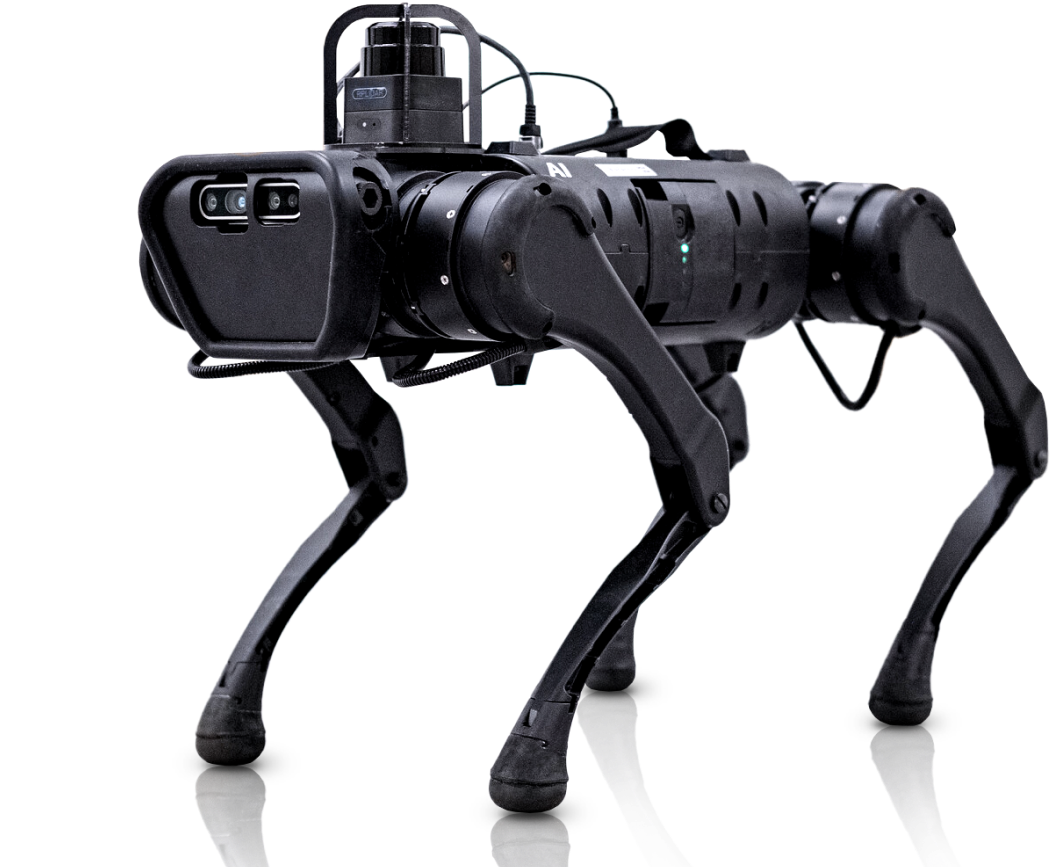
\includegraphics[width=\textwidth]{unitree.png}
			\caption{Четырёхногий робот Unitree A1}
			\end{figure}
	\end{minipage}
	\hfill
	\begin{minipage}[t]{0.47\linewidth}
		\textbf{Составная \\ подпись 2}
		
	\end{minipage}
\end{frame}

\begin{frame}
    \frametitle{Управление шагающими роботами}
	\begin{figure}
	\centering
	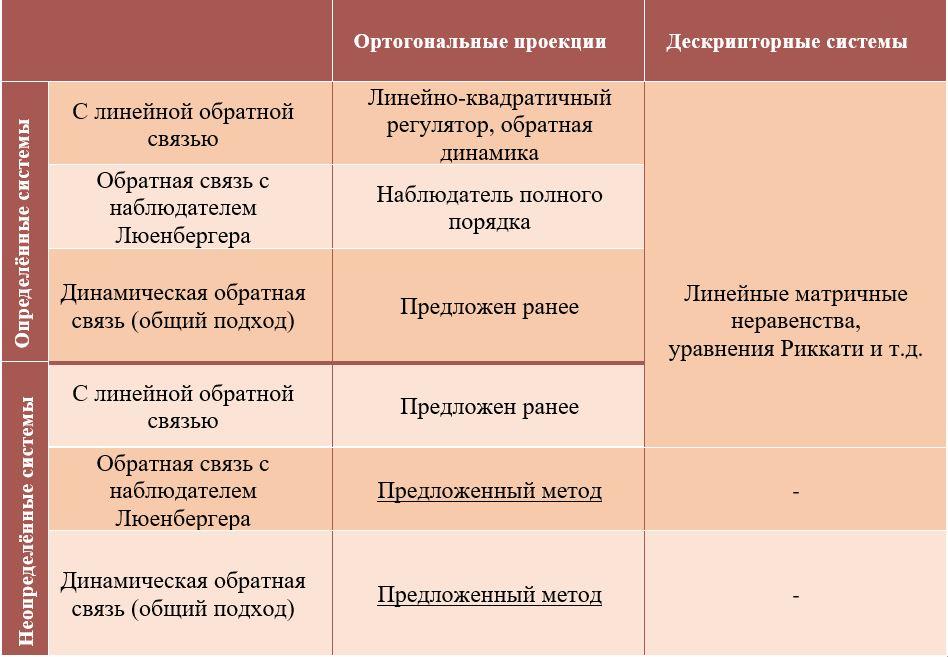
\includegraphics[scale=0.6]{images/table.JPG}
	\caption{Методы управления и наблюдения для систем с механическими ограничениями.}
	\label{fig:table}
\end{figure}
\end{frame}

\subsection{Область исследования}

\begin{frame}
    \frametitle{Предмет и объект исследования}
	Объектом исследования является оптимальное робастное управление шагающими роботами с параметрическими неопределённостями.
	\vfill
	Предметом исследования являются методы математического моделирования системы с неопределённостями, описывающие динамику шагающего робота и численные методы с использованием ортогональных методов и линейных матричных неравенств для нахождения коэффициентов регулятора и наблюдателя с последующими вычислениями при помощи комплекса программ.
\end{frame}

\subsection{Цели и задачи}

\begin{frame}
    \frametitle{Цели и задачи}
    Целью диссертационной работы является разработка численных ортогональных методов оптимального робастного управления математическими моделями, описывающих шагающих роботов, с использованием линейных матричных неравенств.
    
	Выполненные задачи:
	\begin{itemize}
		\item Проведён обзор литературы;
		\item Описана математическая модель шагающего робота;
		\item Предложен численный метод оптимального робастного управления для систем с параметрическими неопределённостями;
		\item Предложен численный метод оптимального робастного управления с динамической обратной связью для системы с аддитивными неопределённостями;
		\item Разработан комплекс программ, реализующий предложенные методы.
	\end{itemize}
\end{frame}

\section{Основная часть}

\subsection{Математическое моделирование}

\begin{frame}
    \frametitle{Ортогональная декомпозиция}
    \centering
\end{frame}

\begin{frame}
	\frametitle{Линеаризация}
	\centering
\end{frame}

\subsection{Методы оптимального робастного управления}

\begin{frame}
    \frametitle{Система с мультипликативными неопределённостями}
    Рассмотрим следующую систему:
    \begin{equation}
    	\label{eq:part2_linear_dynamics}
    	\begin{cases}
    		\dot z=({A}_n+\Delta {A}_n)z + ({B}+\Delta {B})u,\\
    		y = ({C}+ \Delta {C}){N}  z.
    	\end{cases}
    \end{equation}
    
    Вводим наблюдатель Люенбергера с состоянием $\hat{z}$:
    %
    \begin{equation}
    	\label{eq:Luenberger}
    	\dot{\hat{z}}={A}_n\hat{z}+{B}u+{L}_z(y- {C} {N}\hat{z}),
    \end{equation}
    %
    где ${L}_z$ --- матрица наблюдателя. 
    
    Рассмотрим следующий закон управления с линейной обратной связью:
    %
    \begin{equation}
    	\label{eq:control_law}
    	u={K}_z\hat{z}.
    \end{equation}
\end{frame}

\begin{frame}
	\frametitle{Система с мультипликативными неопределённостями}
	После введения ошибки как $e_z=z-\hat{z}$, получаем систему:
	\begin{equation}
		\label{eq:part2_system}
		\begin{bmatrix}
			\dot{z} \\ \dot{e}_z
		\end{bmatrix}=\begin{bmatrix}
			({A}_n+\Delta {A}_n +{B}{K}_z+\Delta {B}{K}_z) & -({B}{K}_z+\Delta {B}{K}_z) \\
			(\Delta {A}_n +\Delta {B}{K}_z-{L}_z\Delta {C}{N}) & ({A}_n-{L}_z{C}{N}-\Delta {B}{K}_z)        \end{bmatrix}\begin{bmatrix}
			z \\ e_z
		\end{bmatrix}.
	\end{equation}
	\begin{block}{Теорема 1}
		Система (\ref{eq:part2_system}) асимптотически стабильна для всех матриц
		$\Delta {A}_n={M}_1{F}_1{N}_1$, 
		$\Delta {B}= {M}_2{F}_2{N}_2$, 
		$\Delta {C} = {M}_3{F}_3{N}_3$,
		где
		${F}_i\T{F}_i\leq \nu_i {I}$ для $i=1,2,3$,
		если существуют такие положительно определённые матрицы ${Q}_1$, ${P}_2$ и положительные скаляры
		$\gamma_1>0$, $\gamma_2>0$, $\gamma_3>0$, $\bar{\mu}_1>0$, $\bar{\mu}_2>0$, $\bar{\mu}_3>0$, и $\epsilon_1 > 0$ такие, чтобы следующее линейное матричное неравенство выполнялось:
	\end{block}
\end{frame}

\begin{frame}
	\frametitle{Система с мультипликативными неопределённостями}
	\begin{block}{Теорема 1. Продолжение}
	\[
\label{eq:lmi1}
\begin{medsize}
	\begin{bmatrix}
		{\Lambda}_1 & 0 & {M}_1 & {M}_2&0 & {Q}_1{N}_1\T & {\Lambda}_3 &{\Lambda}_4 & {B}\hat{{K}}_z & 0\\
		* & {\Lambda}_2 & {P}_2{M}_1 & {P}_2{M}_2 & \hat{{L}}_z{M}_3& 0& 0&0&0&{I} \\
		* & * & -\gamma_1{I} & 0&0&0&0&0&0&0\\
		* & * &*  & -\gamma_2{I}&0&0&0&0&0&0\\
		*& * & * &*  & -\gamma_3{I}&0&0&0&0&0\\
		* &* & * & * & *&-\bar{\mu}_1{I}&0&0&0&0\\
		* & * & * &*& *&*&-\bar{\mu}_2{I}& 0&{N}_2\hat{{K}}_z&0\\
		*&*&* &* & * & * & *&-\bar{\mu}_3{I}&0&0\\
		* & * & *&*&* & *&*&*&-\frac{1}{\epsilon_1}{Q}_1&0\\
		* & * & * & *&*&*&*&*&*&-\epsilon_1{Q}_1\\
	\end{bmatrix}<0, \end{medsize}\]
%
где
%
\begin{align*}
	&\hat{{K}}_z={K}_z{Q}_1, \qquad \hat{{L}}_z={P}_2{L}_z, \\
	&{\Lambda}_1={Q}_1{A}_n\T+{A}_n{Q}_1+{B}\hat{{K}}_z+\hat{{K}}_z\T{B}\T, \\
	&{\Lambda}_2={A}_n\T{P}_2+{P}_2{A}_n-\hat{{L}}_z{C}{N}-{N}\T{C}\T\hat{{L}}_z\T, \\
	&{\Lambda}_3=\hat{{K}}_z\T{N}_2\T, \qquad {\Lambda}_4={Q}_1{N}\T{N}_3\T.
\end{align*}
	\end{block}
\end{frame}

\begin{frame}
	\frametitle{Управление с динамической обратной связью}
	Рассмотрим следующую систему:
	\begin{equation}
		\label{eq:part5_linear_dynamics}
		\begin{cases}
			\dot z={A}_n {z} + {A}_r {\zeta} + {B} {u},\\
			y = {C} {N} {z} + {C} {R} {\zeta},
		\end{cases}
	\end{equation}
	где матрицы $A_n$,  $B$ и $C$ являются матрицами состояния, управления и наблюдения соответственно. Матрица ${A}_r$ отвечает за статическую часть матрицы состояния.
	
	Рассмотрим следующий закон управления с динамической обратной связью:
	\begin{equation}
		\label{eq:part5_controller}
		\begin{cases}
			\dot{{z}}_K = {A}_K {z}_K + {B}_K {y},\\
			{u} = {C}_K {z}_K + {D}_K {y}.
		\end{cases}
	\end{equation}
\end{frame}

\begin{frame}
	\frametitle{Управление с динамической обратной связью}
		Объединим уравнения \eqref{eq:part5_linear_dynamics} и \eqref{eq:part5_controller} и получим систему:
	\begin{align}
		\label{eq:part5_cl}
		&\begin{bmatrix}
			{\dot{z}} \\ {\dot{z}}_K 
		\end{bmatrix}
		=
		\begin{bmatrix}
			{A}_N + {B}{D}_K{C}{N} & {B}{C}_K \\
			{B}_K{C}{N} &{A}_K
		\end{bmatrix}
		\begin{bmatrix}
			{z} \\ {z}_K 
		\end{bmatrix}
		+
		\begin{bmatrix}
			{A}_R + {B}{D}_K{C}{R}\\ {B}_K{C}_R
		\end{bmatrix}
		{\zeta}.
	\end{align}
	\begin{block}{Теорема 3}
		Система \eqref{eq:part5_cl}  асимптотически устойчива, если существуют положительно определённые матрицы ${Q}_1>0$, ${P}_1>0$, матрицы $\hat{{A}}_K$,  $\hat{{B}}_K$, $\hat{{C}}_K$ и $D_K$
		и положительный скаляр $\alpha>0$ такие, что выполняется следующие линейные матричные неравенства:
		\[
		\begin{medsize}
			\begin{bmatrix}
				{\Theta}_1  & {A}_N + {\hat{A}}_K\T +{B}{D}_K{C}{N} & {A}_R + {B}{D}_K{C}{R}\\
				\cdots & {\Theta}_2 & {P}_{1}{A}_R + {P}_{1}{B}{D}_K{C}{R}+{P}_1{B}_K{C}{R}\\
				\cdots & \cdots & 0 
			\end{bmatrix} < 
			\begin{bmatrix}
				0 & 0\\
				0 & \alpha {I}
			\end{bmatrix},
		\end{medsize}\]
		\begin{align*}
			\begin{bmatrix} 
				{Q}_{1} & I \\ 
				I & {P}_{1}
			\end{bmatrix} > 0,
		\end{align*}
	\end{block}
\end{frame}

\begin{frame}
	\frametitle{Управление с динамической обратной связью}
	\begin{block}{Теорема 3. Продолжение}
	\begin{align*}
		&{\Theta}_1 = {A}_N{Q}_{1} +{Q}_{1}{A}_N\T + {B}{\hat{C}}_K +{\hat{C}}_K\T{B}\T, \\
		&{\Theta}_2 = {P}_{1}{A}_N +{A}_N\T{P}_{1}+{\hat{B}}_K{C}{N}+{N}\T{C}\T{\hat{B}}_K\T.
	\end{align*}
	
	И коэффициенты регулятора находятся следующим образом 
	\begin{align*}
		&{P}_{2} = ({I}-{P}_{1}{Q}_{1}){Q}_{2}^{-\top},\\
		&{C}_K = ({\hat{C}}_K - {D}_K {C} {N} {Q}_{1} ){Q}_{2}^{-\top},\\
		&{B}_K = {P}_{2}^{-1}({\hat{B}}_K- {P}_{1}{B}{D}_K),\\
		&{A}_K = {P}_{2}^{-1}({\hat{A}}_K-{P}_{1}({A}_N+{B}{D}_K{C}{N}){Q}_{1} -\\ 
		& - {P}_{2}{B}_K{C}{N}{Q}_{1}-{P}_{1} {B}{C}_K{Q}_{2}\T){Q}_{2}^{-\top}.
	\end{align*}
\end{block}
\end{frame}

\begin{frame}
	\frametitle{Описание шагающего робота}
	Используется плоская модель четвероногого робота \textit{Unitree A1} (робот описывается в одном горизонтальном и одном вертикальном измерении), как показано на рисунке \ref{fig:flat_robot},
	\begin{figure}
		\centering
		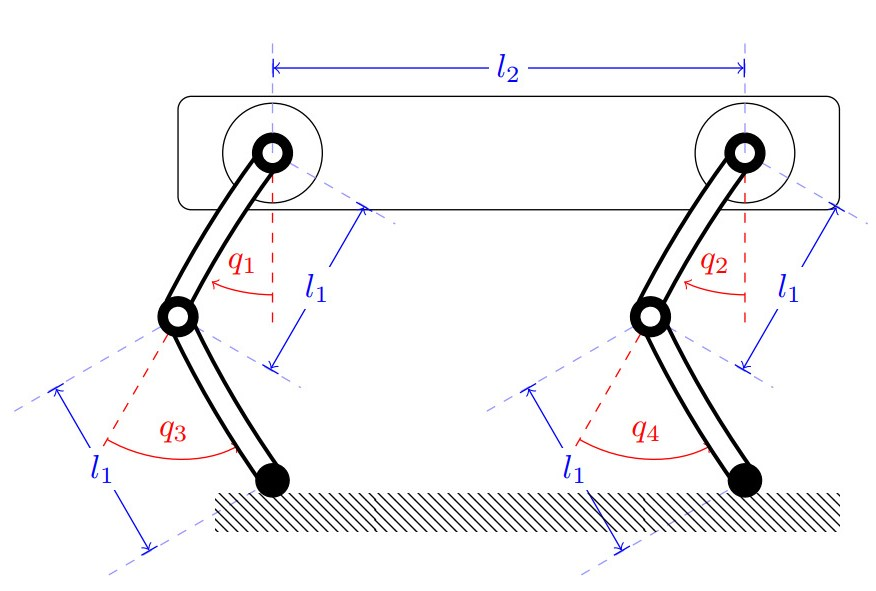
\includegraphics[width=0.7\linewidth]{images/FlatQuadruped.jpeg}
		\caption{Схема плоского четвероногого робота}
		\label{fig:flat_robot}
	\end{figure}
\end{frame}

\begin{frame}
	\frametitle{Целевая функция}
	Неопределённости ограничены следующим образом:
	%
	\begin{equation}
		{F}_i\T{F}_i\leq \nu_i {I}, \ \ i=1,2,3,
	\end{equation}
	где $\nu_i$ --- радиусы неопределённости --- скаляры, определяющие ограничения, накладываемые на нормы ${F}_i$. 
	
	$\mu_i=\gamma_i\nu_i$ для $i=1,2,3$.
	$\bar{\mu}_i=\frac{1}{\mu_i}$
	В отличие от предыдущей задачи оптимизации, здесь не существует естественной формулировки целевой функции. Предлагается два варианта целевой функции:
	\begin{align}
		\label{eq:cost_lin}
		J_\text{lin} &= \sum_{i=1}^{3}\left(\bar{\mu}_i+\gamma_i\right), \\ 
		\label{eq:cost_quad}
		J_\text{quad} & =  \sum_{i=1}^{3}\left((\bar{\mu}_i-\varpi)^2+(\gamma_i-\varpi)^2\right) + \varpi^2,
	\end{align}
	%
	где $\varpi$ --- свободная переменная. Целью обеих целевых функций является максимизация $\nu_i$, которая достигается минимизацией либо $J_\text{lin}$, либо $J_\text{quad}$. Максимизируя $\nu_i$, достигается устойчивость к большему набору неопределённых матриц $\Delta {A}_n$, $\Delta {B}$ и $\Delta {C}$.
\end{frame}

\begin{frame}
	\frametitle{Применение методов}
	Выбираем линейную целевую функцию, задача оптимизационного управления приобретает вид:
	%
	\begin{equation}
		\label{eq:thm4_OCP}
		\begin{aligned}
			& \underset{\bar{\mu}_i,\gamma_i,{Q}_1, {P}_2,\hat{{K}} , \hat{{L}} }{\text{минимизируя}}
			& &  \sum_{i=1}^{3}\left(\bar{\mu}_i+\gamma_i\right), \\
			& \text{при ограничениях}
			& & \begin{cases}
				{Q}_1>0, \ \
				{P}_2>0, \ \
				\bar{\mu}_i>0, \ \
				\gamma_i>0, \ \
				\text{для} \ \ i=1,2,3; \\
				\text{условие из Теоремы 1 }.
			\end{cases}
		\end{aligned}
	\end{equation}
	%
	Данная задача оптимизации имеет параметр $\epsilon_1$ который мы можем найти решетчатым поиском.
\end{frame}

\begin{frame}
	\frametitle{Применение методов}
	\begin{figure}
		\centering
		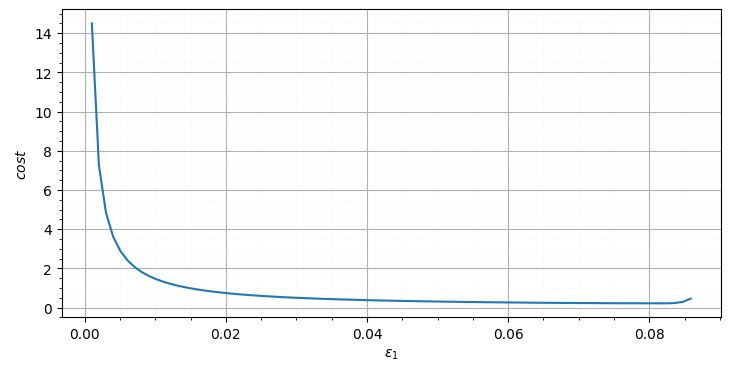
\includegraphics[scale=0.85]{images/mult_soft_cost_qp_eps.JPG}
		\caption{Значение целевой функции задачи оптимального управления \eqref{eq:thm4_OCP}, решённой для плоского четвероногого робота, построенное относительно параметра $\epsilon_1$; обе оси без единиц.}
		\label{fig:cost}
	\end{figure}
\end{frame}

\begin{frame}{Применение методов}
	\begin{figure}
		\centering
		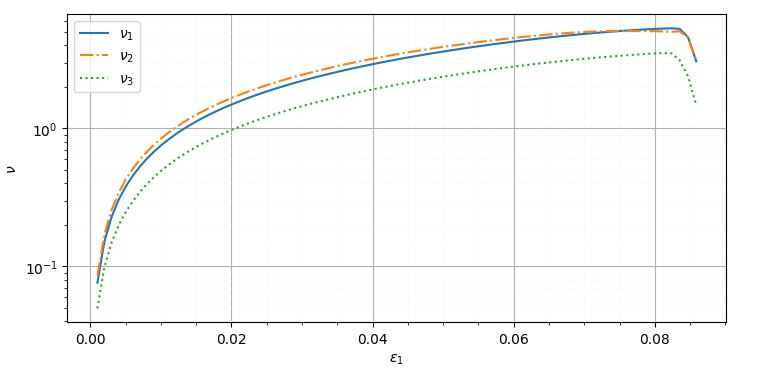
\includegraphics[scale=0.8]{images/mult_soft_nu_eps_qp.JPG}
		\caption{Верхняя граница радиусов неопределённости $\nu_i$ задачи \eqref{eq:thm4_OCP}; графики построены относительно значения свободного параметра $\epsilon_1$; вертикальная ось масштабирована логарифмически, обе оси без единиц.}
		\label{fig:cost_qp}
	\end{figure}
\end{frame}

\subsection{Комплексы программ}

\section{Заключение}
\begin{frame}[plain, noframenumbering]
    \begin{center}
        \Huge
        Остальное
    \end{center}
\end{frame}

\subsection{Формулы}

\begin{frame}
    \frametitle{Формулы}
    \[
    \left\{
    \begin{array}{rl}
        \dot x = & \sigma (y-x)  \\
        \dot y = & x (r - z) - y \\
        \dot z = & xy - bz
    \end{array}
    \right.
    \]
\end{frame}

\begin{frame}
    \frametitle{amsmath}
    \centering
    \begin{minipage}[t]{0.5\linewidth}
        \begin{multline*}
            y = 1 x^1 + 2 x^2 + 3 x^3 + \\ + 4 x^4 + 5 x^5 + \dots
        \end{multline*}
    \end{minipage}
\end{frame}

\begin{frame}[allowframebreaks]
    \frametitle{Уравнения Максвелла}
    \centering{
        \small
        \def\arraystretch{1.8}%
        \begin{tabular}{ll}
            \toprule
            Интегральная форма                                                                                                                                            & Дифференциальная форма                                                          \\ \midrule
            \(Q_e(t) = \displaystyle\oiint_S \vec D(t) \cdot d\vec{s} = \displaystyle\iiint_V \rho_v(t) dv\)                                                              & \(\nabla \cdot \vec D(t) = \rho_v(t)\)                                          \\
            \(\displaystyle\oiint_S \vec B(t) \cdot d\vec{s} = 0\)                                                                                                        & \(\nabla \cdot \vec B(t) = 0\)                                                  \\
            \(V_{emf}(t) = \displaystyle\oint_L \vec E(t) \cdot d\vec{l}\) = \(- \displaystyle\iint_S \left[\frac{\partial\vec{B}(t)}{\partial t}\right] \cdot d\vec{s}\) & \(\nabla \times \vec E(t) = - \frac{\partial\vec{B}(t)}{\partial t}\)           \\
            \(I(t) = \displaystyle\oint_L \vec H(t) \cdot d\vec{l} = \displaystyle\iint_S \left[\vec J(t) + \frac{\partial\vec{D}(t)}{\partial t}\right] \cdot d\vec{s}\) & \(\nabla \times \vec H(t) = \vec J(t) + \frac{\partial\vec{D}(t)}{\partial t}\) \\ \midrule
            \(\displaystyle\oiint_S \vec J \cdot d\vec{s} = -\frac{\partial Q_e}{\partial t}\)                                                                            & \(\nabla \cdot \vec J = - \frac{\partial \rho_v}{\partial t}\)                  \\
            \bottomrule
            \multicolumn{2}{c}{\(\vec D(t) = \left[\varepsilon(t)\right] * \vec E(t)\)}                                                                                                                                                                     \\
            \multicolumn{2}{c}{\(\vec B(t) = \left[\mu(t)\right] * \vec H(t)\)}                                                                                                                                                                             \\
        \end{tabular}
    }
    \framebreak

    \hspace{0.05\linewidth}
    \centering{
        \small
        \def\arraystretch{1.8}%
        \begin{tabular}{ll}
            \toprule
            Интегральная форма                                                                                                                & Дифференциальная форма                               \\ \midrule
            \(Q_e = \displaystyle\oiint_S \vec D \cdot d\vec{s} = \displaystyle\iiint_V \rho_v dv\)                                           & \(\nabla \cdot \vec D = \rho_v\)                     \\
            \(\displaystyle\oiint_S \vec B \cdot d\vec{s} = 0\)                                                                               & \(\nabla \cdot \vec B = 0\)                          \\
            \(V_{emf} = \displaystyle\oint_L \vec E \cdot d\vec{l}\) = \(- \displaystyle\iint_S \left[j \omega \vec B\right] \cdot d\vec{s}\) & \(\nabla \times \vec E = - j \omega \vec B\)         \\
            \(I = \displaystyle\oint_L \vec H \cdot d\vec{l} = \displaystyle\iint_S \left[\vec J + j \omega \vec D\right] \cdot d\vec{s}\)    & \(\nabla \times \vec H = \vec J + j \omega \vec{D}\) \\ \midrule
            \(\displaystyle\oiint_S \vec J \cdot d\vec{s} = - j \omega Q_e\)                                                                  & \(\nabla \cdot \vec J = - j \omega \rho_v\)          \\
            \bottomrule
            \multicolumn{2}{c}{\(\vec D(t) = \left[\varepsilon\right] \vec E(t)\)}                                                                                                                   \\
            \multicolumn{2}{c}{\(\vec B(t) = \left[\mu\right] \vec H(t)\)}                                                                                                                           \\
        \end{tabular}
    }
\end{frame}

\subsection{Таблицы}

\begin{frame}
    \frametitle{Таблица}
    \centering
    \begin{tabular}{|l|l|}
        \hline
        \textbf{Заголовок 1} & \textbf{Заголовок 2} \\
        \hline
        Сумма                & \(b+a\)              \\
        \hline
        Разность             & \(a-b\)              \\
        \hline
        Произведение         & \(a*b\)              \\
        \hline
    \end{tabular}
\end{frame}

\begin{frame}
    \frametitle{Другая таблица}
    \centering
    \begin{tabular}{lc}
        \toprule
        \multicolumn{1}{c}{\textbf{Заголовок 1}} & \textbf{Заголовок 2} \\ \midrule
        Сумма                                    & \(b+a\)              \\
        Разность                                 & \(a-b\)              \\
        Произведение                             & \(a*b\)              \\
        \bottomrule
    \end{tabular}
\end{frame}


\subsection{Разное}

\begin{frame}
    \frametitle{Большой многоуровневый список}
    \begin{itemize}
        \item \textbf{Пункт 1}
              \begin{itemize}
                  \itemi Подпункт 1-1
                  \itemi Подпункт 1-2
              \end{itemize}
        \item \textbf{Пункт 2}
              \begin{itemize}
                  \itemi Подпункт 2-1
              \end{itemize}
        \item \textbf{Пункт 3}
              \begin{itemize}
                  \itemi Подпункт 3-1
                  \itemi Подпункт 3-2
              \end{itemize}
        \item \textbf{Пункт 4}
              \begin{itemize}
                  \itemi Подпункт 4-1
              \end{itemize}
        \item \textbf{Пункт 5}
              \begin{itemize}
                  \itemi Подпункт 5-1
                  \itemi Подпункт 5-2
                  \itemi Подпункт 5-3
              \end{itemize}
    \end{itemize}
\end{frame}

\begin{frame}
    \frametitle{Четыре изображения}
    \centering
    \includegraphics[width=0.35\linewidth,angle=35]{latex}
    \includegraphics[width=0.35\linewidth,angle=135]{latex}\\
    \includegraphics[width=0.35\linewidth,angle=15]{latex}
    \includegraphics[width=0.35\linewidth,angle=-15]{latex}
\end{frame}

